\documentclass[sigconf,review]{acmart}
\setcopyright{acmlicensed}
\AtBeginDocument{
  \providecommand\BibTeX{{\normalfont B\kern-0.5em{\scshape i\kern-0.25em b}\kern-0.8em\TeX}}
}
\copyrightyear{2026}
\acmYear{2026}
\acmConference[CIKM '26]{The 35th ACM International Conference on Information and Knowledge Management}{November 7--11, 2026}{Rome, Italy}
% \acmBooktitle{CIKM '26: The 35th ACM International Conference on Information and Knowledge Management, November 7--11, 2026, Rome, Italy}

\usepackage{booktabs}
\usepackage{amsmath}
\usepackage{amsfonts}
\usepackage{graphicx}
\usepackage{placeins}
\usepackage{tikz}
\usetikzlibrary{arrows.meta,positioning,fit,backgrounds,calc}
\usepackage{xspace}
\usepackage{float}
\usepackage{xcolor}

\newcommand{\bench}{\textsc{FInject}\xspace}

\begin{document}

\title{\bench: Expanding Finance Reasoning Problems through Injection of Unanswerability}

\author{Jinkyu Kim}
\authornote{These authors contributed equally to this work.}
\orcid{0000-0001-9484-7541}
\affiliation{
  \institution{Fanding}
  \city{Seoul}
  \country{Republic of Korea}
}
\email{jkcost2511@gmail.com}

\author{Jinsu Kim}
\authornotemark[1]
\affiliation{
  \institution{Pusan National University}
  \city{Busan}
  \country{Republic of Korea}
}
\email{jinsu.kim@pusan.ac.kr}

\author{Wooik Park}
\authornotemark[1]
\affiliation{
  \institution{Pusan National University}
  \city{Busan}
  \country{Republic of Korea}
}
\email{wipark@pusan.ac.kr}

\author{Mujeen Sung}
\affiliation{
  \institution{Kyung Hee University}
  \city{Yongin}
  \country{Republic of Korea}
}
\email{mujeensung@khu.ac.kr}

\author{Mogan Gim}
\orcid{0000-0002-6458-7723}
\affiliation{
  \institution{Hankuk University of Foreign Studies}
  \city{Yongin}
  \country{Republic of Korea}
}
\email{gimmogan@hufs.ac.kr}

\author{Donghee Choi}
\authornote{Corresponding author.}
\orcid{0000-0002-8857-9680}
\affiliation{
  \institution{Pusan National University}
  \city{Busan}
  \country{Republic of Korea}
}
\email{dchoi@pusan.ac.kr}

\renewcommand{\shortauthors}{Kim et al.}


\begin{abstract}
Financial reasoning benchmarks typically assume that every problem is answerable once a model performs the right calculation.
Real financial documents are less tidy. 
Material values may be missing, silently dropped, duplicated with incompatible figures, or contradicted across sources, rendering the underlying numerical problem unsolvable.
We introduce \bench, a benchmark for unanswerability detection in financial decision-making.
% We pair answerable controls with human-validated unanswerable variants built through a six-way perturbation taxonomy.
Each instance is a human-validated unanswerable variant built through a six-way perturbation taxonomy, paired with an answerable control.
We use a paired metric rewarding correct answers on originals and refusals on unanswerable variants, plus a metacognitive score balancing refusal quality and hallucination avoidance.
Experiments show that \bench discriminates evidence-aware reasoning from surface accuracy, separating models that abstain appropriately from those that either hallucinate on unanswerable variants or over-refuse, distinctions that answerable-only benchmarks cannot reveal.
\bench provides a reusable dataset, unanswerability injection protocol, annotation guideline, and evaluation harness for studying abstention in high-stakes numerical reasoning.
Code and data are publicly available at \url{https://github.com/pnu-clink/finject} and \url{https://huggingface.co/datasets/pnu-clink/finject} (DOI: \href{https://doi.org/10.57967/hf/9057}{10.57967/hf/9057}).
\end{abstract}

\keywords{Financial NLP, Benchmark, Abstention, Hallucination, Numerical Reasoning, Large Language Models}

\ccsdesc[500]{Computing methodologies~Natural language processing}
\ccsdesc[300]{Information systems~Data mining}

\maketitle


\section{Introduction}


\begin{figure}[H]
\centering
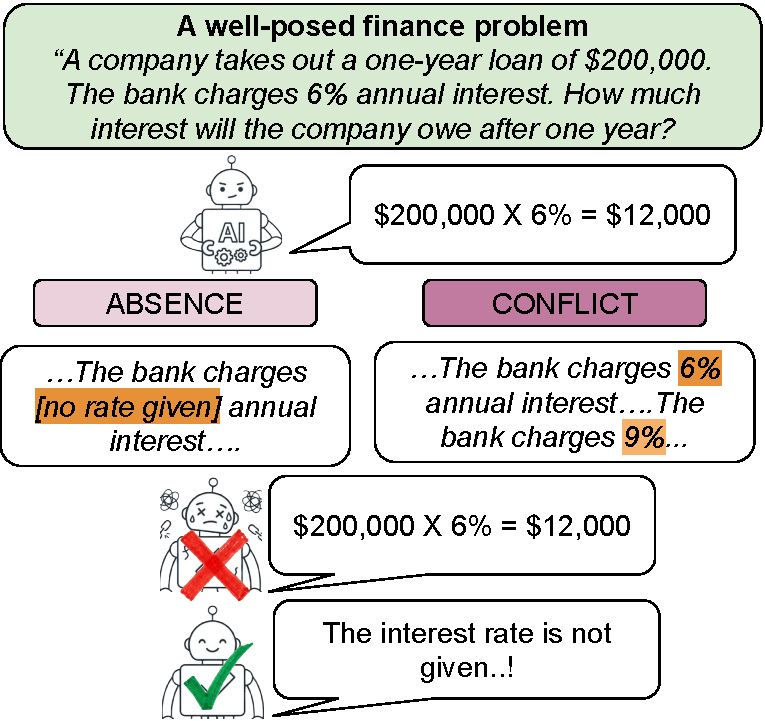
\includegraphics[width=0.7\columnwidth]{figures/teasor.pdf}
\caption{\bench turns a well-posed finance problem into absence and conflict variants, separating models that hallucinate an answer from those that correctly abstain.}
\label{fig:concept}
\end{figure}

\begin{figure*}[t]
\centering
\scriptsize
\resizebox{0.8\textwidth}{!}{%
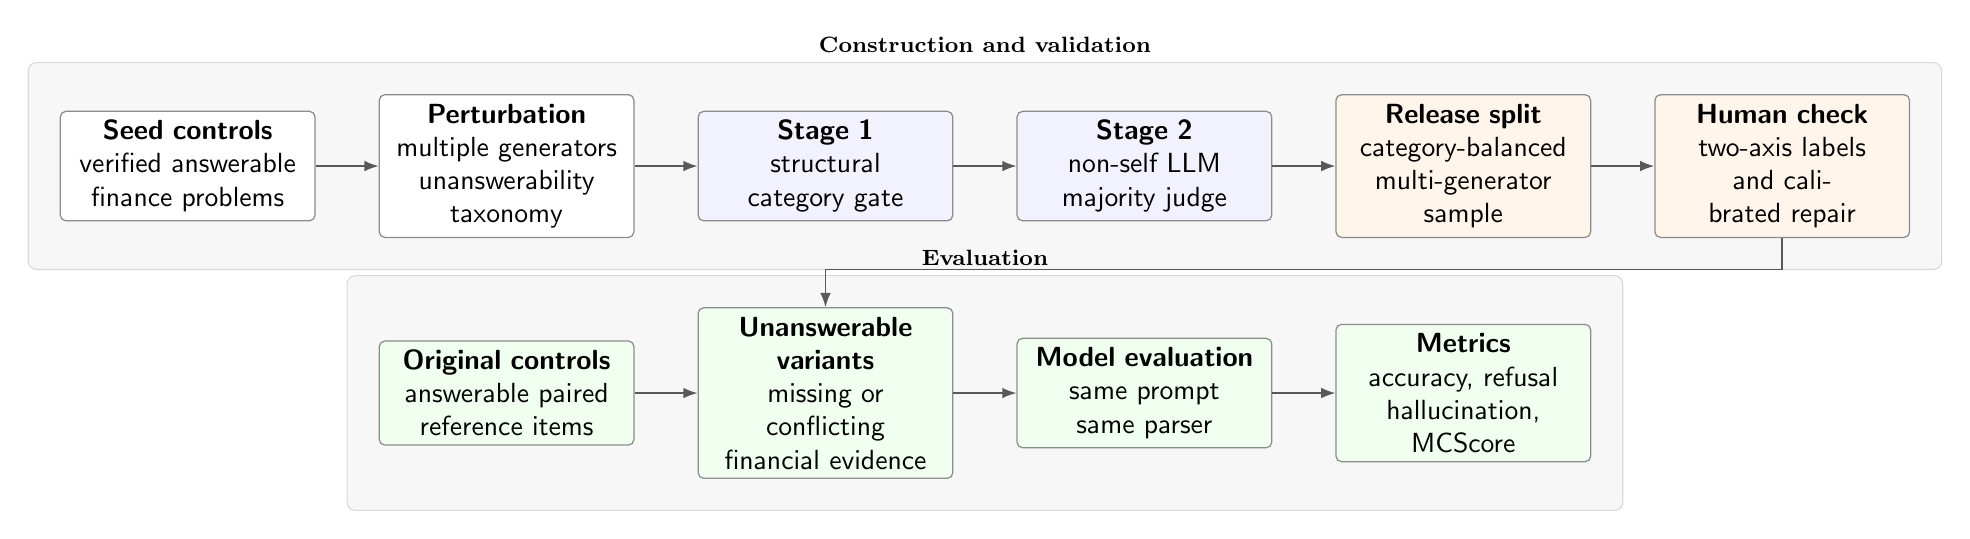
\begin{tikzpicture}[
  font=\sffamily,
  node distance=7mm and 8mm,
  stage/.style={
    draw=black!45,
    rounded corners=2pt,
    line width=.45pt,
    align=center,
    minimum height=11mm,
    text width=30mm,
    fill=white
  },
  gate/.style={stage, fill=blue!5},
  sample/.style={stage, fill=orange!8},
  eval/.style={stage, fill=green!6},
  arrow/.style={-{Latex[length=1.8mm]}, line width=.55pt, draw=black!65},
  band/.style={draw=black!15, rounded corners=3pt, fill=black!3}
]
\node[stage] (seed) {\textbf{Seed controls}\\verified answerable\\finance problems};
\node[stage, right=of seed] (gen) {\textbf{Perturbation}\\multiple generators\\unanswerability taxonomy};
\node[gate, right=of gen] (stageone) {\textbf{Stage 1}\\structural\\category gate};
\node[gate, right=of stageone] (stagetwo) {\textbf{Stage 2}\\non-self LLM\\majority judge};
\node[sample, right=of stagetwo] (sample) {\textbf{Release split}\\category-balanced\\multi-generator sample};
\node[sample, right=of sample] (human) {\textbf{Human check}\\two-axis labels\\and calibrated repair};

\node[eval, below=13mm of gen] (orig) {\textbf{Original controls}\\answerable paired\\reference items};
\node[eval, right=of orig] (neg) {\textbf{Unanswerable variants}\\missing or conflicting\\financial evidence};
\node[eval, right=of neg] (model) {\textbf{Model evaluation}\\same prompt\\same parser};
\node[eval, right=of model] (metrics) {\textbf{Metrics}\\accuracy, refusal\\hallucination, MCScore};

\draw[arrow] (seed) -- (gen);
\draw[arrow] (gen) -- (stageone);
\draw[arrow] (stageone) -- (stagetwo);
\draw[arrow] (stagetwo) -- (sample);
\draw[arrow] (sample) -- (human);
\draw[arrow] (human.south) -- ++(0,-4mm) -| (neg.north);
\draw[arrow] (orig) -- (neg);
\draw[arrow] (neg) -- (model);
\draw[arrow] (model) -- (metrics);

\begin{scope}[on background layer]
\node[band, fit=(seed)(gen)(stageone)(stagetwo)(sample)(human), inner sep=4mm,
  label={[font=\bfseries\footnotesize]above:Construction and validation}] {};
\node[band, fit=(orig)(neg)(model)(metrics), inner sep=4mm,
  label={[font=\bfseries\footnotesize]above:Evaluation}] {};
\end{scope}
\end{tikzpicture}
}
\caption{\bench construction and evaluation pipeline. Seed problems are first verified as answerable controls, converted into finance-specific unanswerability-injected types, filtered by structural and semantic validation, sampled into a category-balanced multi-generator release, and finally evaluated as paired original-control and unanswerable-instance tasks.}
\Description{A left-to-right pipeline diagram showing seed controls, perturbation generation, Stage 1 structural validation, Stage 2 non-self judge validation, balanced sampling, human checking and repair, downstream evaluation, and final metrics.}
\label{fig:pipeline}
\end{figure*}


In real-world corporate enterprises, financial situations are tightly intertwined with \textbf{decision-making processes} (e.g., investment evaluation, risk management), where each decision can affect multiple aspects of business management, such as asset liquidity and sustainable profitability. Effective financial decision making requires an accurate assessment of the given situation, together with complex reasoning and problem-solving skills. However, some financial situations may either present \textit{insufficient context} or contain \textit{contradictory information}, rendering the underlying numerical problems unsolvable. Therefore, it is important to preemptively assess the answerability of the problem itself, before producing answers that may lead to disastrous decisions. 



Large language models (LLMs) are increasingly deployed in financial tasks as core decision-support systems, owing to their strong reasoning capabilities and, more recently, their use within agentic systems. 
Because each LLM-generated response can directly affect investment, credit, audit, and risk decisions, robust standards and benchmarks are essential for helping practitioners apply LLMs reliably. 
Moreover, evaluating LLMs with respect to their mathematical problem-solving skills, their potential to expand their financial knowledge, and their reasoning capabilities lies at the core of deploying an agentic financial decision-making system.
Existing financial reasoning benchmarks such as FinQA, TAT-QA, and FinanceReasoning measure LLMs' numerical reasoning by having them answer finance-related questions~\cite{chen2021finqa,zhu2021tatqa,financereasoning2025}. 
To the best of our knowledge, \textbf{however, none of these benchmarks assess an LLM's ability to refuse unanswerable questions}.


\bench addresses this gap by turning well-solved financial reasoning problems into \textbf{controlled unanswerable instances}.
We use the hard problems of FinanceReasoning and select 78 seed problems that are solved by a strong majority of baseline models.
This selection avoids a trivial negative benchmark where models fail because the original problem was already too difficult.
We then perturb each seed using a taxonomy grounded in financial document failures: explicit missing values, silent omissions, intra-document value conflicts, inter-source conflicts, and mutually exclusive premises.
Every resulting instance is finally validated by human annotators, ensuring that FInject serves as a reliable, human-verified dataset.

Through experiments with \bench, we show that even strong financial reasoners with high answerable-question accuracy frequently hallucinate on unanswerable variants, and that our proposed metric, which couples correct answers on originals with correct refusals on unanswerable variants, distinguishes selective abstention from indiscriminate over-refusal. 
We further find that our perturbation taxonomy captures distinct construction and verification bottlenecks, motivating a validated multi-generator pool over single-model outputs.

Our contributions are:
\begin{itemize}
  \item \textbf{Dataset.} A financial unanswerability benchmark built from 78 answerable seed problems and their controlled unanswerable variants.
  \item \textbf{Taxonomy.} A six-way perturbation taxonomy separating absence detection from conflict detection.
  \item \textbf{Evaluation protocol.} Three tasks that measure whether models abstain, identify why they should abstain, and explain the evidence gap.
  \item \textbf{Quality controls.} Human verification guidelines with independent labels for category fidelity and unanswerability.
\end{itemize}
Figure~\ref{fig:pipeline} summarizes the construction, validation, repair, and downstream evaluation workflow.

\section{Related Resources}

Unanswerable QA benchmarks such as SQuAD 2.0 and AbstentionBench test whether models withhold answers under insufficient evidence~\cite{rajpurkar2018know,kirichenko2026abstentionbench}. Conflict-oriented resources such as ConflictBank, ContraDoc, and FaithEval study inconsistent evidence and context faithfulness~\cite{su2024conflictbank,li2024contradoc,ming2025faitheval}. In finance, FinQA, TAT-QA, and FinanceReasoning focus on answerable numerical reasoning~\cite{chen2021finqa,zhu2021tatqa,financereasoning2025}, while FinS-Pilot evaluates financial RAG systems where relevant information is expected to exist~\cite{finspilot2025}. Recent resources also emphasize fine-grained hallucination evaluation and metrics~\cite{cfaith2025,mirage2025}. \bench combines these directions: it keeps financial numerical reasoning as the base task, but makes evidence insufficiency and irreconcilability the object of evaluation.

\section{Construction}

\subsection{Overview of \bench}

\bench turns answerable financial numerical reasoning problems into controlled unanswerable variants. We select seeds from FinanceReasoning, whose finance word problems pair a question and context with a numeric answer and executable reasoning procedure~\cite{financereasoning2025}. Four generator families---Claude Opus, GPT-5.5, Gemini 2.5 Pro, and R1-Distill-32B---inject six types of unanswerability, after which candidates pass through structural validation, non-self semantic judging, balanced sampling, and human verification with repair.

\begin{figure}[t]
  \centering
  % 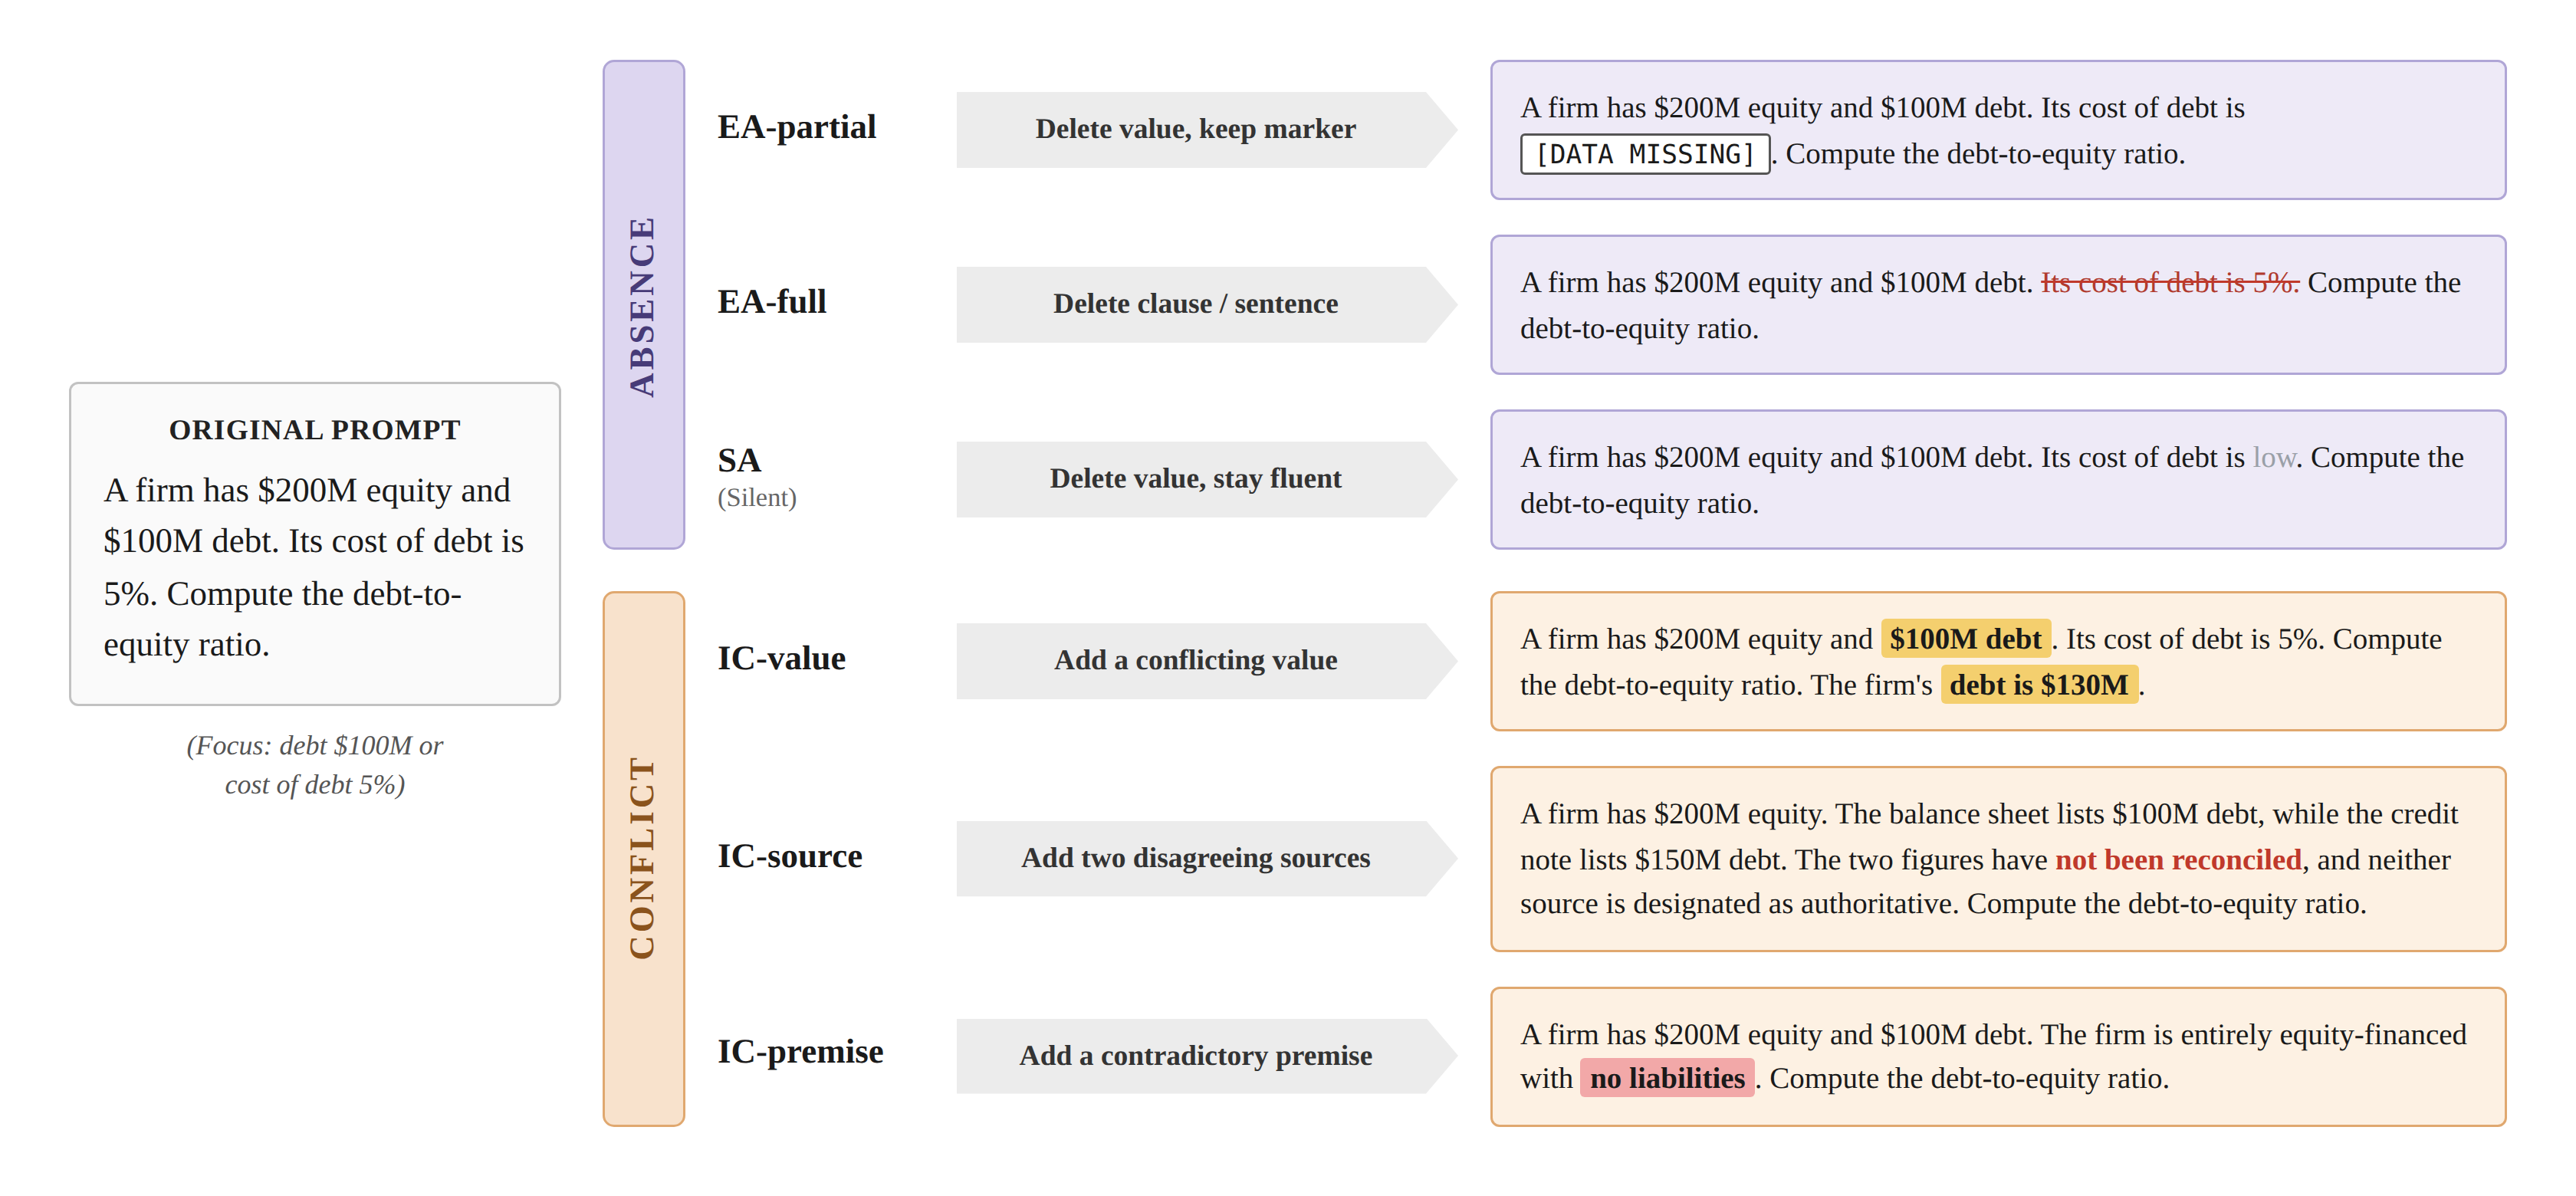
\includegraphics[width=\columnwidth]{figures/taxonomy.png}
  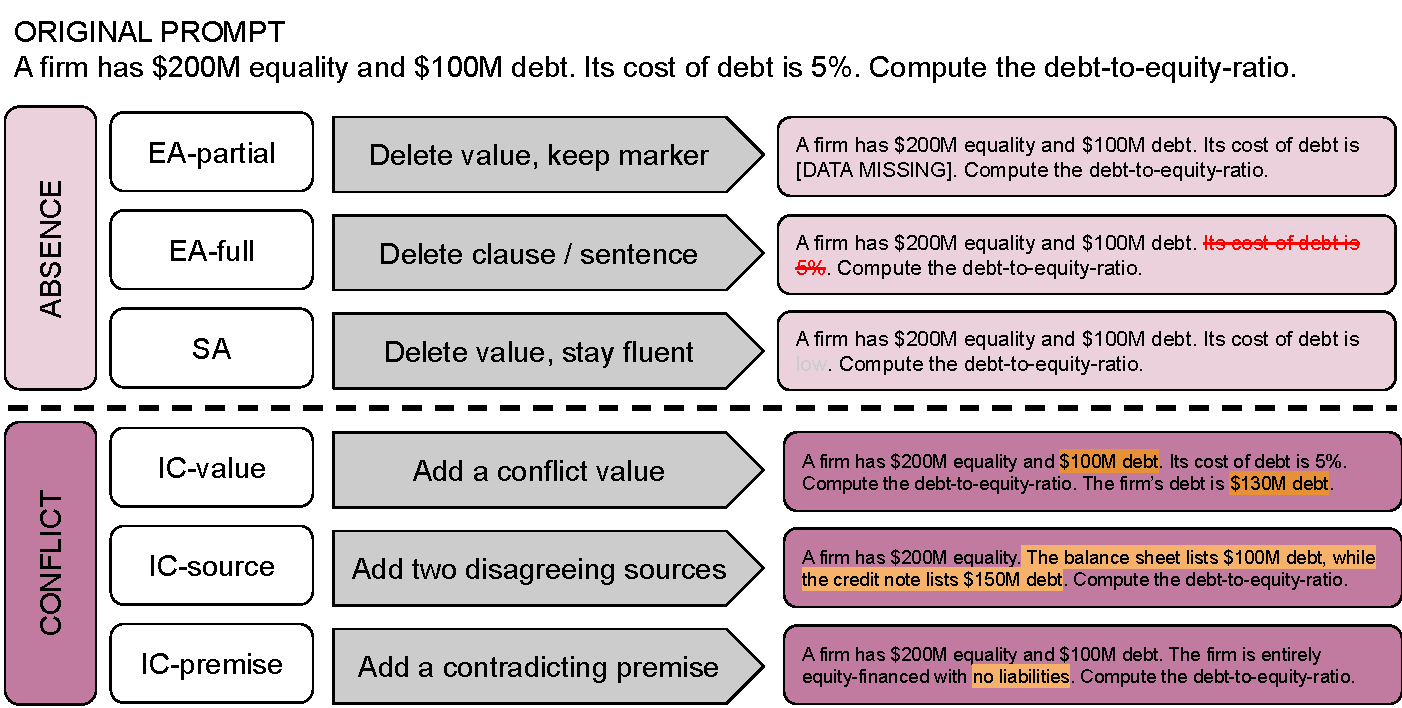
\includegraphics[width=0.8\columnwidth]{figures/taxonomy2.pdf}
  \caption{Illustration of taxonomy}
  \label{fig:variation}
\end{figure}

\subsection{Seed Problems}

We use 78 hard-split FinanceReasoning seeds whose original answers are verified through blind solving and executable reference solutions, avoiding a trivial benchmark where models fail because the original calculation is already too difficult. A value, premise, or source choice is \emph{answer-critical} if it is used by the executable solution and is necessary to derive the unique numeric answer.

\subsection{Perturbation Taxonomy}

For each seed, four generator families produce one candidate for each of six categories, yielding $78 \times 6 \times 4 = 1{,}872$ candidates before validation. \ref{item:taxanomy} summarizes the taxonomy.

% \begin{table}[t]
% \centering
% \small
% \caption{\bench perturbation taxonomy.}
% \label{tab:taxonomy}
% \scalebox{0.75}{
% \begin{tabular}{@{}p{0.4\columnwidth}p{0.75\columnwidth}@{}}
% \toprule
%  \textbf{Type} & \textbf{Manipulation methods} \\
% \midrule
% % multiline Absence
%  Partial Removal   (A-partial, AP) & Replace an answer-critical value with a visible marker \\
%  Silent Absence (A-silent, AS) & Remove a value without an explicit marker \\
%  Full Removal (A-full, AF) & Delete the carrier clause, sentence, or row \\
%  % Silent Absence (A-silent, AS) & Remove a value without an explicit marker \\
 
% \midrule 
% % Multiline Conflict
%  Adding Conflict of Value (C-value, CValue ) & State the same quantity with conflicting values \\
%  Source Conflict (IC-source, CS) & Attribute conflicting values to named sources \\
%  Premise Conflict (IC-premise, CP) & Add mutually incompatible premises \\
%  \textbf{IC-premise} & Information Conflict,  Add mutually incompatible premises \\
% \bottomrule
% \end{tabular}
% }
% \end{table}

The absence categories remove answer-critical evidence. The conflict categories preserve enough apparent evidence to make the question look answerable, but introduce two plausible alternatives without a reliable preference cue. We explicitly reject conflicts resolved by audit status, recency, management confirmation, action anchors, or definitional arithmetic.

\subsection{Two-Stage Automatic Validation}

Recent LLM benchmark studies pair generation with systematic verification~\cite{kung2026leapsuperchargingllmsformal,cheng2025travelbench,liu2026autoresearchclaw,lee2026selfverifieddistillation}. We therefore use a two-stage automatic validation pipeline: Stage~1 checks the visible form required by each perturbation type, while Stage~2 checks whether the structurally valid edit removes a uniquely supported answer.



% \begin{table}[t]
% \centering
% \small
% \caption{\bench perturbation taxonomy.}
% \label{tab:taxonomy}
% \scalebox{0.75}{
% \begin{tabular}{@{}p{0.4\columnwidth}p{0.75\columnwidth}@{}}
% \toprule
%  \textbf{Type} & \textbf{Manipulation methods} \\
% \midrule
% % multiline Absence
%  Partial Removal   (A-partial, AP) & Replace an answer-critical value with a visible marker \\
%  Silent Absence (A-silent, AS) & Remove a value without an explicit marker \\
%  Full Removal (A-full, AF) & Delete the carrier clause, sentence, or row \\
%  % Silent Absence (A-silent, AS) & Remove a value without an explicit marker \\
 
% \midrule 
% % Multiline Conflict
%  Adding Conflict of Value (C-value, CValue ) & State the same quantity with conflicting values \\
%  Source Conflict (IC-source, CS) & Attribute conflicting values to named sources \\
%  Premise Conflict (IC-premise, CP) & Add mutually incompatible premises \\
%  \textbf{IC-premise} & Information Conflict,  Add mutually incompatible premises \\
% \bottomrule
% \end{tabular}
% }
% \end{table}

\textbf{Stage~1} is a deterministic structural gate.
It uses rule-based schema, marker, deletion, and conflict-pattern checks before any semantic judging. These predicates do not decide whether the edited value is truly necessary or whether a conflict is resolvable; they only remove malformed or wrong-shape candidates:
\begin{itemize}
\label{item:taxanomy}
  \item \textbf{EA-partial (Explicit Absence-partial)}: Replace an answer-critical value with a visible marker. exactly one \texttt{[DATA MISSING]} marker appears in place of a numeric value.
  \item \textbf{EA-full (Explicit Absence-full)}: one carrier sentence, clause, or table row is removed and no explicit marker remains.
  \item \textbf{SA (Silent Absence)}: a numeric value is removed or neutralized while the surrounding prose or table remains fluent and marker-free.
  \item \textbf{IC-value (Information Conflict-value)}: two different numeric values appear for the same quantity label.
  \item \textbf{IC-source (Information Conflict-source)}: two named sources attribute different values to the same quantity.
  \item \textbf{IC-premise (Information Conflict-premise)}: an additional premise is inserted as a condition on the same calculation rather than as a replacement answer.
\end{itemize}
Candidates that fail these structural predicates are excluded before Stage~2. Across the 1,872 generated candidates, 1,690 pass Stage~1 when malformed, empty, or unevaluated cells are counted as structural failures.
Table~\ref{tab:stage1} reports the current construction audit.

\begin{table}[!t]
\centering
\small
\caption{Stage~1 structural pass rates before semantic judging.}
\label{tab:stage1}
\begin{tabular}{lrr}
\toprule
\textbf{Generator} & \textbf{Pass} & \textbf{Macro pass rate} \\
\midrule
Claude Opus & 446/468 & 95.3 \\
GPT-5.5 & 440/468 & 94.0 \\
Gemini 2.5 Pro & 410/468 & 87.6 \\
R1-Distill-32B & 394/468 & 84.2 \\
\bottomrule
\end{tabular}
\vspace{2pt}

% \footnotesize{Rates use all generated candidates as the denominator; malformed, empty, or unevaluated cells count as failures. The supplementary material reports the accounting check connecting Stage~1 to the downstream candidate pool.}
\end{table}
% \FloatBarrier


\textbf{Stage~2} is a semantic judge gate over the Stage~1 survivors. It decides what Stage~1 leaves open: whether the edited evidence is answer-critical and whether the remaining context still supports a unique answer. Judges label category validity and unanswerability. Absence candidates pass only if the removed evidence is required by the reference solution and is not recoverable from the remaining text; conflict candidates pass only if the alternatives concern the same answer-critical quantity or premise and are not resolved by priority cues, action anchors, unit conversion, or back-derivation. To reduce generator-family bias, each candidate is judged only by non-self model families. The main Stage~2 decision is:
\[
  \mathrm{Stage2Pass}(x)=
  \mathbb{1}\left[\sum_{j \in J_x}
  \mathbb{1}(\mathrm{Unanswerable}_j(x)=\mathrm{PASS}) \ge 2\right],
\]
where $J_x$ is the set of eligible non-self judges. The main automatic criterion is:
\[
  \mathrm{FinalPass}(x)=\mathrm{Stage1Pass}(x) \land \mathrm{Stage2Pass}(x).
\]
Judges also emit a category-validity label. We use it for strict sensitivity analysis rather than as the main automatic criterion, because Stage~1 already enforces structural category conformance:
\[
  \mathrm{StrictPass}(x)=
  \mathrm{Stage1Pass}(x) \land
  \mathbb{1}\left[\sum_{j \in J_x}s_j(x)\ge2\right],
\]
where $s_j(x)=1$ only if judge $j$ assigns PASS to both category validity and unanswerability.

\subsection{Release Sampling and Human Verification}

We use generator pass rates to characterize the construction pool, but sample the release split from the automatic $\mathrm{FinalPass}$ union rather than from the strongest generator. For each category, we collect source problem identifiers with at least one automatic-pass candidate. The bottleneck categories, IC-source and IC-premise, contain 71 such identifiers before release sampling, so we set the per-category target to 71 and construct a balanced 426-instance split. Sampling is without replacement within each category, and when multiple generators provide a candidate for the same source and category, we choose one by deterministic quota-balanced assignment with fixed seed 20260603.

Human verification is then applied to the sampled candidates. The interface hides automatic judge outputs and generator identity, but shows the original problem, perturbed problem, intended category, and Python solution. Annotators label \emph{category validity} and \emph{unanswerability} independently; candidates rejected by both assigned annotators are repaired or regenerated before release. The supplementary material reports the Stage~2 matrix, agreement statistics, repair counts, and representative failures.



\section{Tasks and Metrics}

\bench supports three tasks: answerability detection, perturbation-type prediction, and rationale generation grounded in the perturbed context. In the main experiments, we focus on answerability detection using 78 answerable controls and 426 unanswerable variants from the final release.

Original accuracy measures whether a model computes the correct numeric answer on answerable controls. Refusal F1 treats correct refusals on unanswerable variants as true positives and over-refusals on answerable controls as false positives. Hallucination rate is the fraction of unanswerable variants for which a model still returns a numeric answer. PairSucc is stricter: a model must answer the paired original correctly and refuse the corresponding unanswerable variant. We summarize abstention quality as $\mathrm{MCScore} =\mathrm{RefusalF1}\times(1-\mathrm{HallucinationRate})$. Full metric formulas, parse-failure handling, and the output schema are reported in the supplementary material.

\section{Experiments}
% \begin{table*}[!t]
\begin{table}[!t]
\centering
\small
\caption{Model answerability evaluation on \bench. Cohere: Cohere Command A, Acc: Orig. Acc., R. F1: Ref. F1, MC: MCScore, PairSucc}
\label{tab:downstream-results}
\scalebox{0.8}{
\begin{tabular}{llrrrrrr}
\toprule
\textbf{Model} & \textbf{Group} & $N_{\mathrm{neg}}$ & \textbf{Acc.}$\uparrow$ & \textbf{R. F1}$\uparrow$ & \textbf{Halluc.}$\downarrow$ & \textbf{MC}$\uparrow$ & \textbf{PS}$\uparrow$ \\
\midrule
GPT-5.5 & gen-family & 320 & 89.7 & 92.1 & 12.5 & 80.6 & 76.9 \\
Claude Opus 4.7 & gen-family & 318 & 85.9 & 89.5 & 18.6 & 72.9 & 68.2 \\
Gemini 2.5 Pro & gen-family & 318 & 82.0 & 91.0 & 16.0 & 76.4 & 69.2 \\
R1-Distill-32B & gen-family & 322 & 66.7 & 78.0 & 35.1 & 50.6 & 45.0 \\
\midrule
Qwen3-8B & disjoint open & 426 & \textbf{94.9} & 80.7 & 32.2 & 54.8 & \textbf{64.6} \\
Llama-3.3-70B & disjoint open & 426 & 25.6 & 86.9 & 18.8 & 70.6 & 18.5 \\
Qwen2.5-72B & disjoint open & 426 & 16.7 & 87.3 & 21.4 & 68.7 & 12.2 \\
DeepSeek V3.1 & disjoint open & 426 & 28.2 & 85.6 & 24.2 & 64.9 & 20.9 \\
Mistral Large & disjoint API & 426 & 34.6 & 90.9 & 14.8 & 77.4 & 31.0 \\
Cohere & disjoint API & 426 & 7.7 & 89.0 & 15.5 & 75.2 & 5.9 \\
Grok 4.20 & disjoint API & 426 & 15.4 & \textbf{94.2} & \textbf{8.2} & \textbf{86.5} & 12.9 \\
\bottomrule
\end{tabular}
}
\vspace{2pt}

% \footnotesize{The top block lists evaluator families also used as perturbation generators; for these rows, same-family negative instances are excluded from $N_{\mathrm{neg}}$. Bold marks the best score among generator-disjoint $N_{\mathrm{neg}}=426$ rows. PairSucc is the primary paired metric. Cohere: Cohere Command A, Acc: Orig. Acc., MC: MCScore}
% \end{table*}
\end{table}


The experiments answer three resource-level questions about what \bench contributes as a benchmark: whether it exposes hallucination in capable financial reasoners, whether it separates calibrated abstention from over-refusal, and whether its perturbation taxonomy captures distinct construction and verification bottlenecks.

\textbf{Q1. Does \bench reveal hallucination in otherwise capable financial reasoners?} Table~\ref{tab:downstream-results} is the main empirical result. It pairs answerable controls with final-release unanswerable variants and tests whether a model can compute when evidence is sufficient but abstain when evidence is missing or irreconcilable. The frontier generator-family rows still hallucinate numeric answers on many eligible unanswerable variants.

Although Qwen3-8B records the highest original-control accuracy (94.9\%), it ranks only \#3 on PairSucc (64.6\%), since it responds to 32.3\% of the unanswerable variants instead of abstaining.
GPT-5.5, Claude Opus 4.7, and Gemini 2.5 Pro hallucinate on 12.5\%, 18.6\%, and 16.0\%, respectively. High original accuracy alone is also insufficient. R1-Distill-32B shows the same over-answering pattern at a lower accuracy range, with 66.7\% original accuracy, 45.0 PairSucc, and 35.1\% hallucination. Thus, \bench exposes an evidence-awareness failure that ordinary answerable finance benchmarks do not isolate.

% \begingroup
% \setlength{\intextsep}{2pt}
% \setlength{\textfloatsep}{2pt}
% \setlength{\abovecaptionskip}{2pt}
% \setlength{\belowcaptionskip}{2pt}
% \endgroup
\begin{table}[H]
\centering
\small
\caption{Validated candidate pool by generator.}
\label{tab:final-matrix}
\scalebox{0.75}{
\begin{tabular}{lrrl}
\toprule
Generator & Macro & Pass & Weakest cat. \\
\midrule
Claude Opus & 90.6 & 424/468 & IC-source\\
Gemini 2.5 Pro & 80.1 & 375/468 & IC-premise\\
GPT-5.5 & 74.6 & 349/468 & IC-source\\
R1-Distill-32B & 66.9 & 313/468 & IC-premise\\
\bottomrule
\end{tabular}
}
\end{table}

\vspace{-0.5cm}
\begin{table}[H]
\centering
\small
\caption{Human verification and repair summary.}
\label{tab:release-human-summary}
\scalebox{0.75}{
\begin{tabular}{lrrr}
\toprule
Category & $N$ & Repaired & Final agr./$\kappa$ \\
\midrule
EA-partial & 71 & 11 & 95.77 / 0.855 \\
EA-full & 71 & 15 & 91.55 / 0.777 \\
SA & 71 & 17 & 91.55 / 0.791 \\
IC-value & 71 & 1 & 95.77 / 0.386 \\
IC-source & 71 & 19 & 90.14 / 0.773 \\
IC-premise & 71 & 7 & 97.18 / 0.859 \\
\midrule
Overall & 426 & 70 & 93.66 / 0.799 \\
\bottomrule
\end{tabular}
}
\end{table}



\textbf{Q2. Does \bench separate abstention from over-refusal?} Table~\ref{tab:downstream-results} also shows why refusal alone is not enough. Refusal-heavy behavior can look good under abstention-only metrics: Grok 4.20 has the best Refusal F1, hallucination rate, and MCScore among generator-disjoint rows, but its original-control accuracy is only 15.4\%, yielding 12.9 PairSucc. This indicates conservative refusal rather than reliable financial reasoning. The paired design of \bench makes this visible because each unanswerable variant is grounded in an answerable original. We therefore treat PairSucc as the strict paired metric: a model receives credit only when it solves the original problem and refuses the corresponding unanswerable variant.



\textbf{Q3. Do perturbation types expose different construction and verification bottlenecks?} Table~\ref{tab:final-matrix} shows that valid candidate availability is uneven across generators and perturbation types. Claude Opus has the highest macro Pass rate, but every generator has a weak category, and conflict categories are the bottleneck. This means the taxonomy is not merely decorative: absence and conflict perturbations create different failure modes for generators and validators, supporting the use of a validated multi-generator pool rather than raw outputs from a single model.


Table~\ref{tab:release-human-summary} shows the same point from the human verification side. Review identifies 70 joint failures among 426 sampled candidates, concentrated in IC-source, SA, and EA-full, and all joint failures are repaired or regenerated before release. These failures reflect finance-specific judgments such as source priority, silent recoverability, and over-deletion. The final inclusion label reaches 93.66\% agreement with Cohen's $\kappa=0.799$. Thus, the released benchmark is not simply an LLM-generated set of fluent edits; it is a validated and repaired resource with explicit provenance and annotation evidence.

\section{Conclusion}

\bench turns answerable financial reasoning problems into controlled tests of whether models know when not to answer. 
This capability is distinct from ordinary financial calculation: models can solve originals yet hallucinate when values are missing or conflicting, while others appear strong only by over-refusing. 
Combining a finance-specific perturbation taxonomy, non-self automatic validation, human repair, and paired abstention metrics, \bench offers a reusable resource for measuring evidence-aware financial reasoning, not answer production alone.

% \bench turns answerable financial reasoning problems into controlled tests of whether models know when not to answer. The experiments show that this capability is distinct from ordinary financial calculation: models can solve original controls yet still hallucinate answers when essential values are missing or evidence is conflicting, while other models can appear strong by refusing too often. By combining a finance-specific perturbation taxonomy, non-self automatic validation, human repair, and paired abstention metrics, \bench provides a reusable resource for measuring evidence-aware financial reasoning rather than answer production alone.

% The dataset, metadata, perturbation prompts, validation scripts, annotation guideline, evaluation harness, and supplementary material are publicly available through the repository and DOI archive given in the Abstract.


\section*{GenAI Usage Disclosure}

The authors used generative AI tools, including OpenAI GPT-family tools, Anthropic Claude-family tools, Google Gemini-family tools, and DeepSeek-R1-Distill-family tools, to assist with code generation, perturbation generation, automatic judging, drafting, editing, and internal consistency checks. All experimental design choices, dataset inclusion decisions, annotation guidelines, labels, paper claims, and final text are reviewed and approved by the authors.

\bench is a diagnostic benchmark, not a financial-advice system; it uses public seed problems and synthetic perturbations, and its current scope is English textual numerical reasoning with controlled single-instance evidence failures.

\bibliographystyle{ACM-Reference-Format}
\bibliography{main}

\end{document}

